\subsection{Experimental Results}
\label{subsec:performanceComparison_results}

%---------------------- ACO VS SSO ---------------------

Table \vref{table:performanceComparison_ACOSSOBEST} presents the average produced results the proposed system (SSO) and the plain ACO implementation has produced. Representation of the best route set, having for routes, produced by SSO is seen in Fig. \vref{fig:bestRouteSet4}. Best, worst, average, and median produced results in addition to the standard deviation can be found in Appendix \ref{appendixC}, Table \vref{table:performanceComparison_ACOFull}.

    \begin{table}[H]
    \centering
    \begin{tabular}{|l||l|l|l|l|l|}
    \hline
    \textbf{System} & \textbf{$d_0(\%)$} & \textbf{$d_1(\%)$} & \textbf{$d_2(\%)$} & \textbf{$d_{unsat}(\%)$} & \textbf{$ATT$} \\
    \hline
    ACO avg & 81.92 & 16.13 & 1.86 & 0.09 & 10.43\\
    \hline
    SSO avg & 85.21 & 13.49 & 1.30 & 0.00 & 10.27\\
    \hline
    \end{tabular}
    \caption {The best route set, having four routes, constructed by the generic ACO implementation and the proposed system.}
    % 50 runs
    \label{table:performanceComparison_ACOSSOBEST}
    \end{table}

   

%-------------------- 4 route sets ---------------------
\begin{figure}[H]
    \begin{center}
    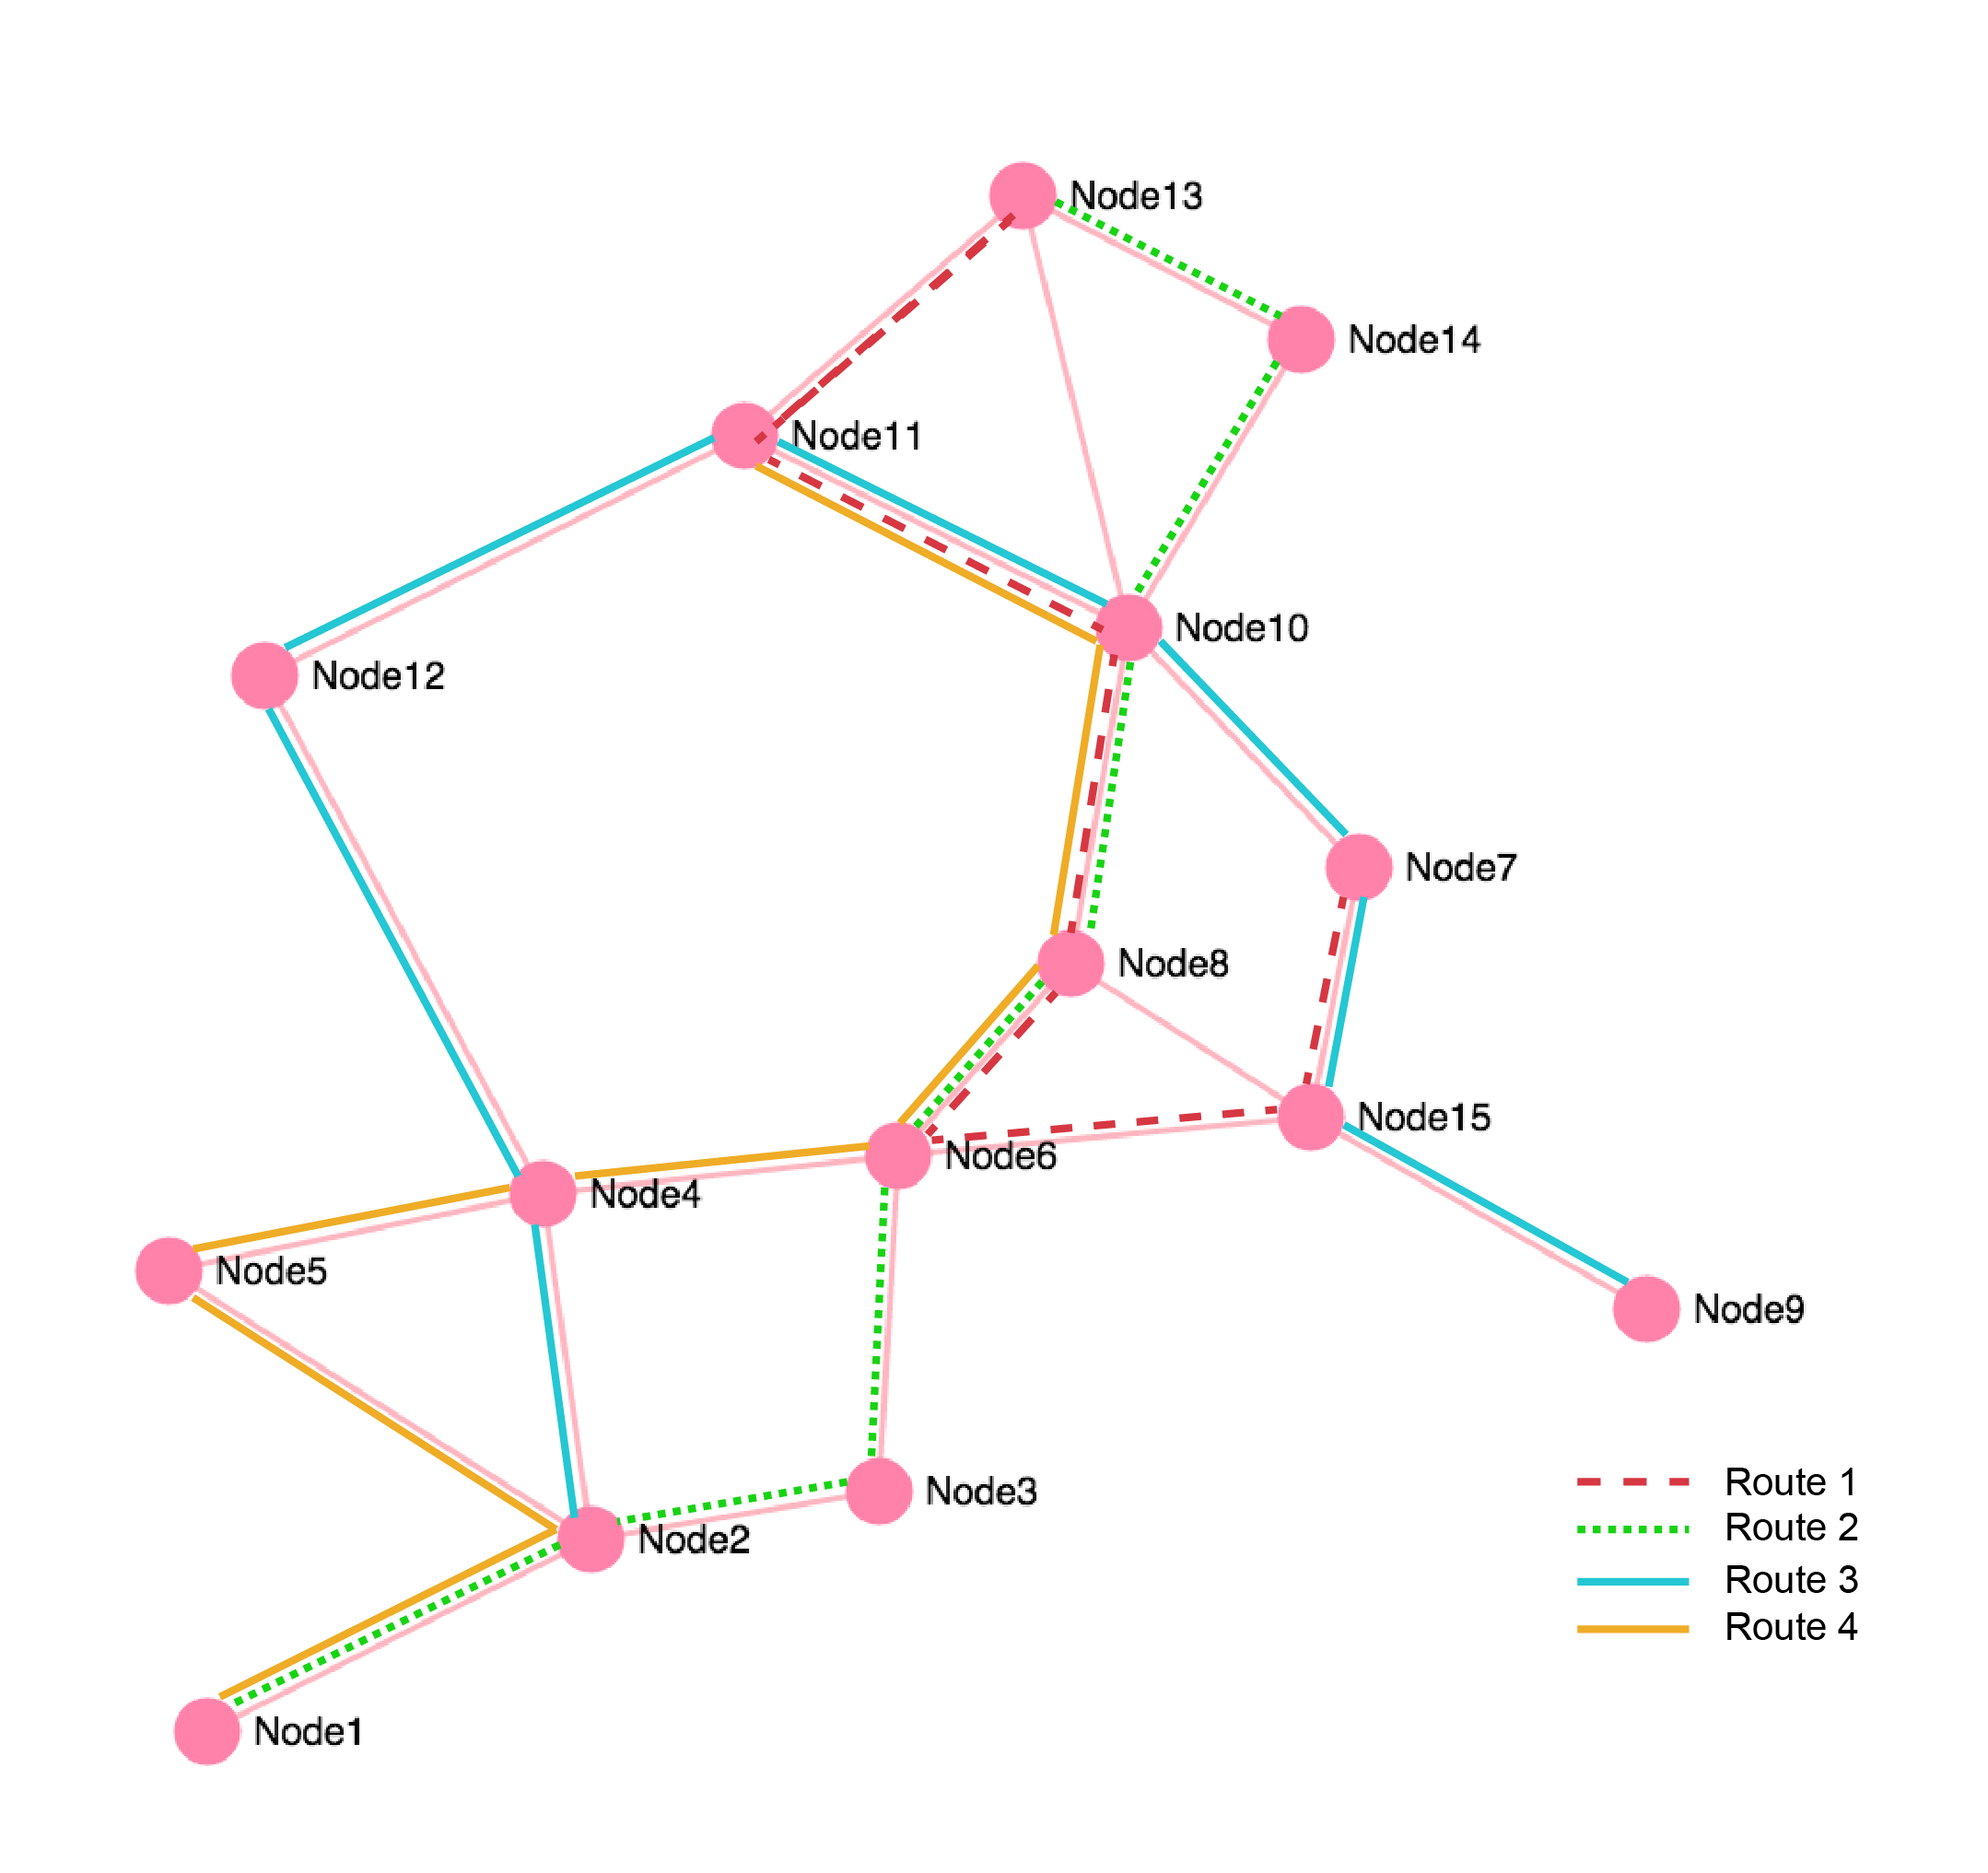
\includegraphics[width=4in]{assets/mandlnetwork_4routes.png}
    \end{center}
    \caption{Illustration of the best route set, having four routes, constructed by the proposed system on Mandl's Network}
    \label{fig:bestRouteSet4} 
\end{figure}

Table \vref{table:performanceComparison_4} presents the results produced by the proposed system, having four routes, and results from route sets constructed by other approaches. The table is sorted in ascending order with respect to the $ATT$ value.

\begin{table}[H]
	\centering
    \hspace*{-1.0cm}
    \begin{tabular}{|l||l|l|l|l|l|}
 	\hline
 	\textbf{System} & $d_0(\%)$ & $d_1(\%)$ & $d_2(\%)$ & $d_{unsat}(\%)$ & $ATT$ \\
 	\hline
    \citet{nikolic14} avg & 95.05 & 4.95 & 0.00 & 0.00 & -$^1$ \\
    \citet{kechagiopoulos14} best & 91.84 & 7.64 & 0.51 & 0.00 & 10.64 \\
    \citet{zhang10} & 91.46 & 8.54 & 0.00 & 0.00 & 10.65 \\
    \citet{kechagiopoulos14} avg & 90.52 & 8.75 & 0.73 & 0.00 & 10.71 \\
    \citet{chew12} best & 93.71 & 6.29 & 0.00 & 0.00 & 10.82 \\
    \citet{chew12} avg & 92.88 & 6.91 & 0.20 & 0.00 & 11.16 \\
    \citet{fan10} best & 93.26 & 6.74 & 0.00 & 0.00 & 11.37 \\
    \citet{fan10} SA$^2$ avg & 92.48 & 7.52 & 0.00 & 0.00 & 11.55 \\
    \citet{fan10} HC$^3$ avg & 91.83 & 8.17 & 0.00 & 0.00 & 11.69 \\
    \citet{chakroborty02} & 86.86 & 12.00 & 1.14 & 0.00 & 11.90 \\
    \citet{kidwai98} & 72.95 & 26.91 & 0.13 & 0.00 & 12.72 \\
    \citet{mandl79} & 69.94 & 29.93 & 0.13 & 0.00 & 12.90 \\
    \hline
    SSO Best & 87.73 & 10.98 & 1.28 & 0.00 & 10.03\\
    SSO Average & 85.21 & 13.49 & 1.30 & 0.00 & 10.27\\
    SSO Median & 85.81 & 13.29 & 1.09 & 0.00 & 10.26\\
    SSO Worst & 76.56 & 22.16 & 1.28 & 0.00 & 10.01\\
    Standard Deviation & 2.66 & 2.70 & 0.84 & - & 0.18\\
    %SSO Confidence interval$^b$ & ~ & ~ & ~ & ~ & ~ \\
    \hline
    \end{tabular}
    \caption {Comparing the best route set, having four routes, produced by the proposed system, with route sets constructed by other approaches.}
    \begin{itemize}[noitemsep]
    %\item[$^a$:] mintues per user
    \item[$^1$:] ATT not supplied
    \item[$^2$:] Simulated Annealing based system
    \item[$^3$:] Hill Climbing based system
    %\item[$^b$:] Confidence Interval with a confidence level of 95\%
    \end{itemize}
    \label{table:performanceComparison_4}
\end{table}

%-------------------- 6 route sets ---------------------
Table \vref{table:performanceComparison_4} presents the results produced by the proposed system, having six routes, and results from route sets constructed by other approaches. The table is sorted in ascending order with respect to the $ATT$ value.

\begin{figure}[H]
    \begin{center}
    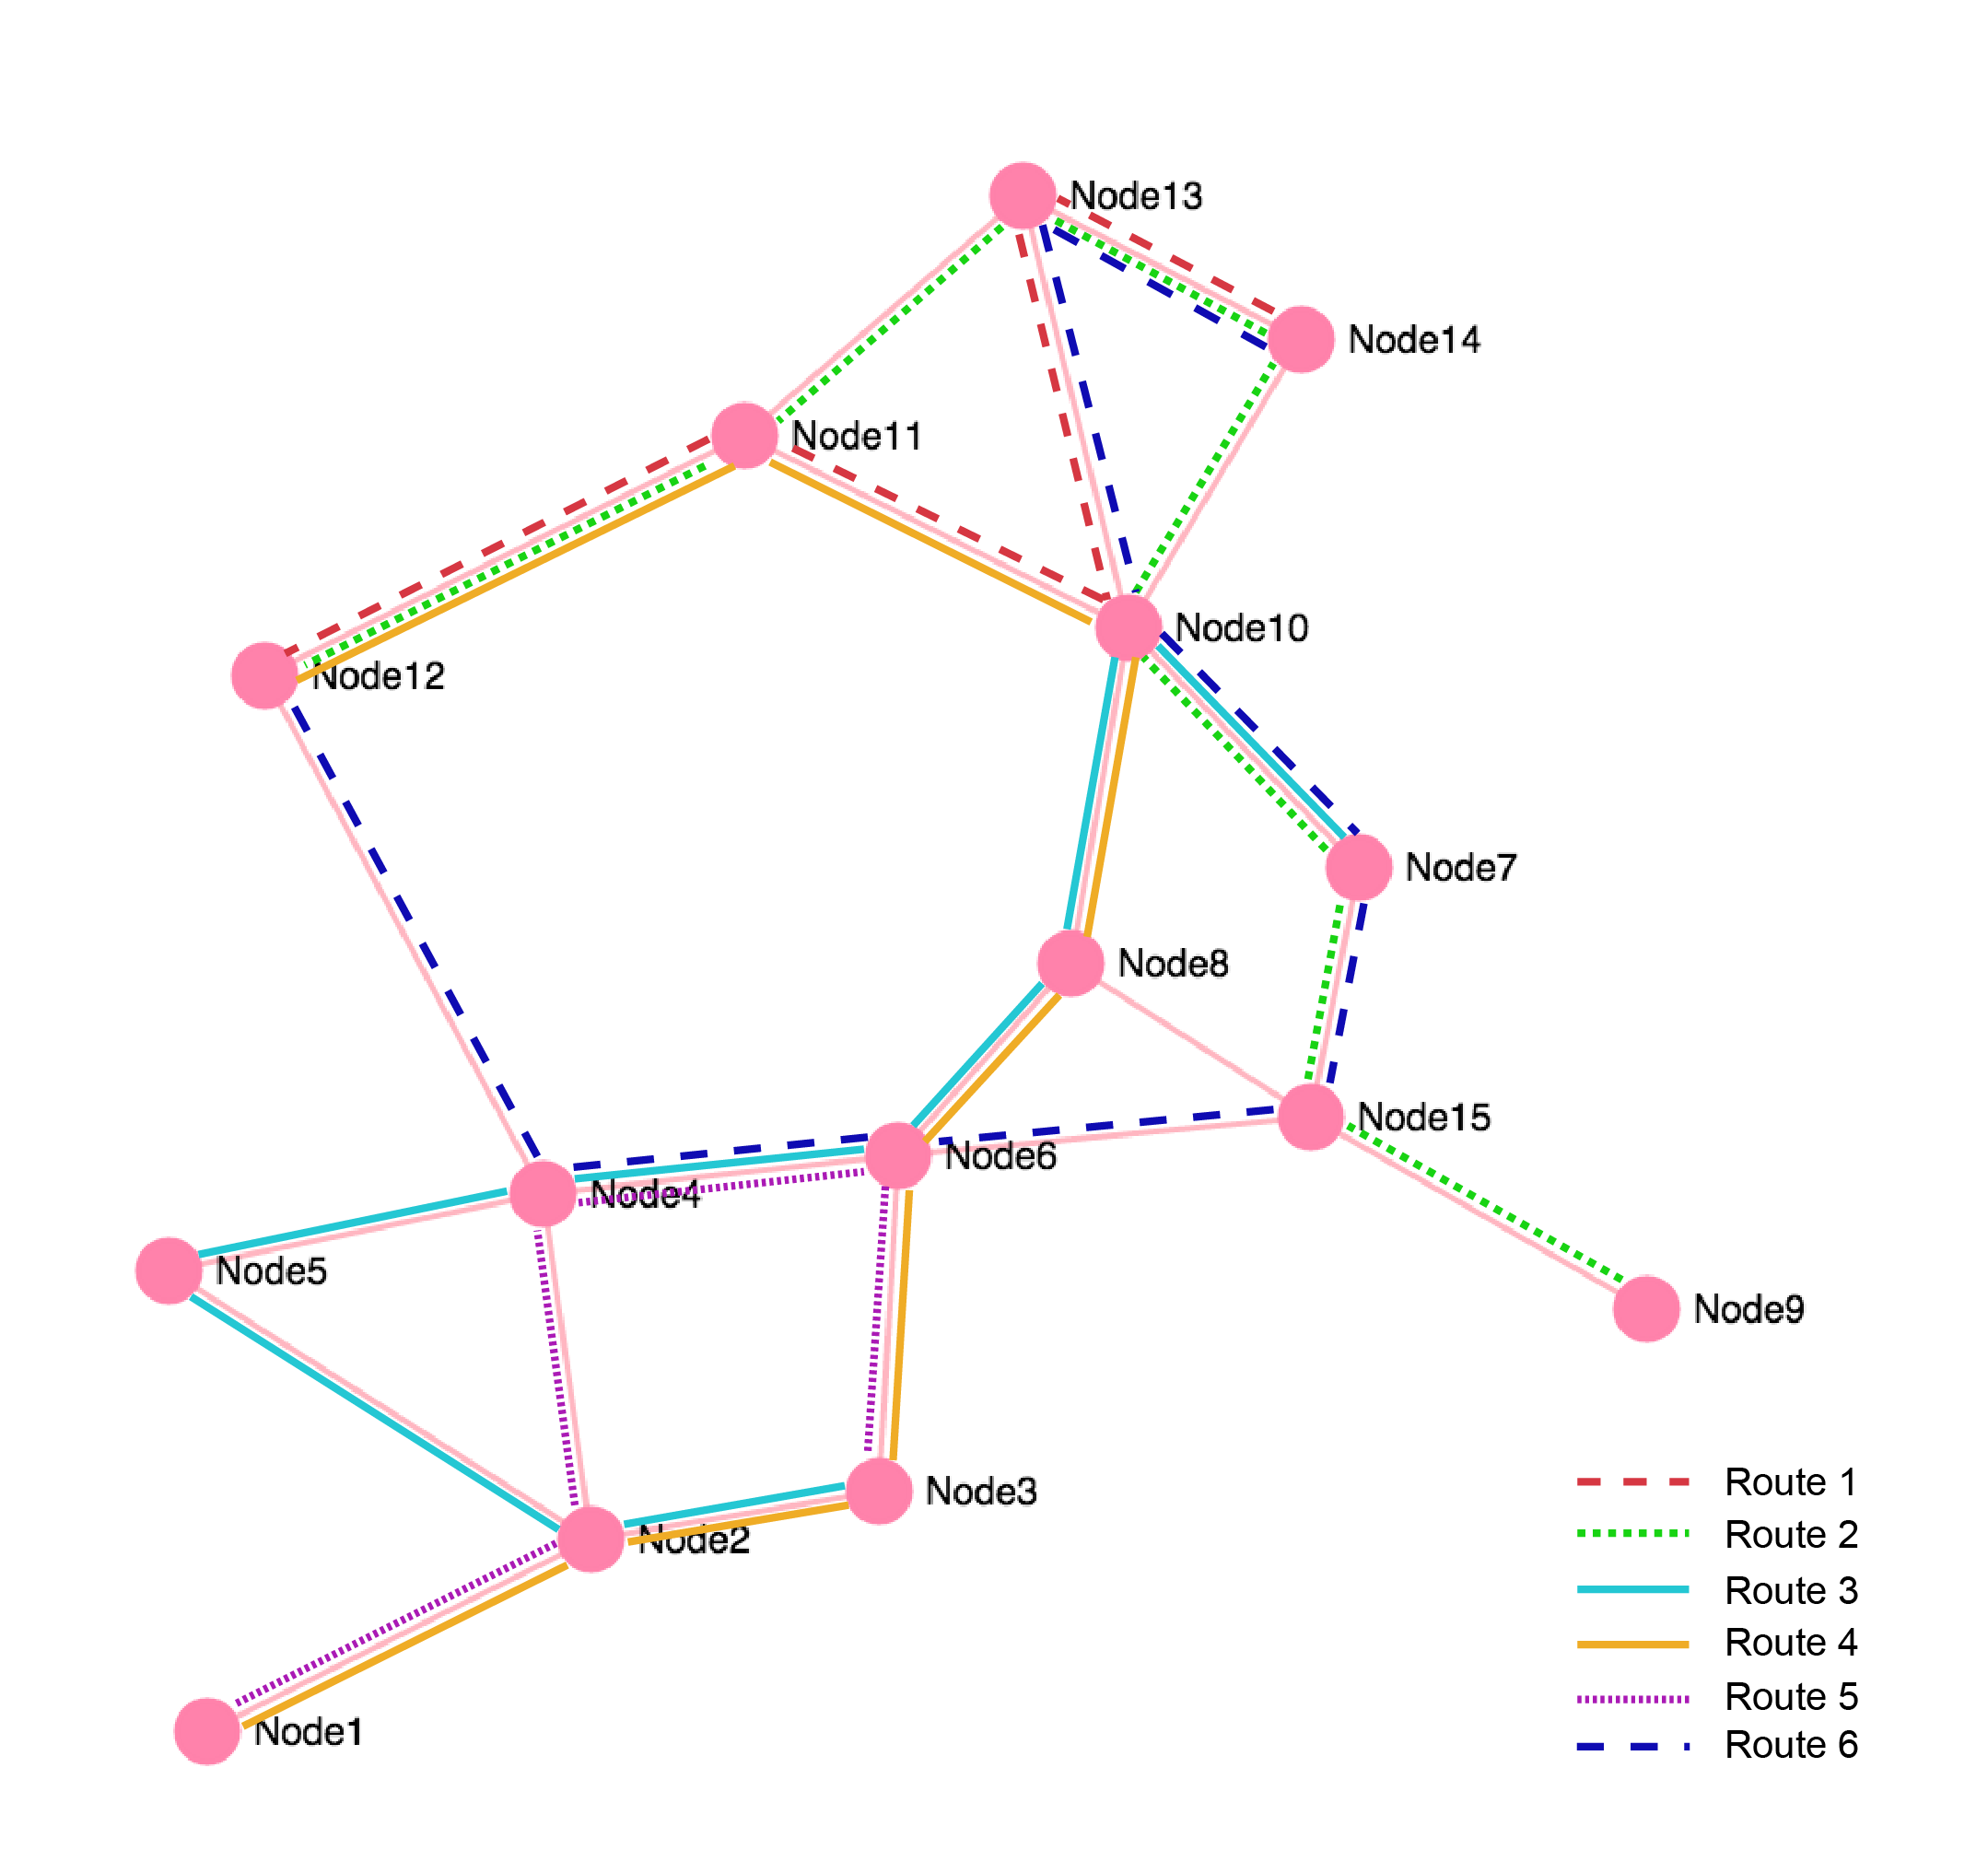
\includegraphics[width=4in]{assets/mandlnetwork_6routes.png}
    \end{center}
    \caption{Illustration of the best route set, having six routes, constructed by the proposed system on Mandl's Network}
    \label{fig:bestRouteSet6} 
\end{figure}

\begin{table}[H]
    \centering
    \hspace*{-1.0cm}
    \begin{tabular}{|l||l|l|l|l|l|}
    \hline
    \textbf{System} & $d_0(\%)$ & $d_1(\%)$ & $d_2(\%)$ & $d_{unsat}(\%)$ & $ATT$ \\
    \hline
    \citet{nikolic14} & 94.34 & 5.65 & 0.00 & 0.00 & - \\
    \citet{kechagiopoulos14} best & 96.21 & 3.47 & 0.32 & 0.00 & 10.23 \\
    \citet{kechagiopoulos14} avg & 95.62 & 4.28 & 0.10 & 0.00 & 10.28 \\
    \citet{chew12} best & 95.57 & 4.43 & 0.00 & 0.00 & 10.28 \\
    \citet{chakroborty02} & 86.04 & 13.96 & 0.00 & 0.00 & 10.30 \\
    \citet{fan10} best & 91.52 & 8.48 & 0.00 & 0.00 & 10.48  \\
    \citet{zhang10} & 91.12 & 8.88 & 0.00 & 0.00 & 10.50 \\
    \citet{chew12} avg & 93.85 & 5.88 & 0.24 & 0.03 & 10.51 \\
    \citet{fan10} SA avg & 90.87 & 8.74 & 0.39 & 0.00 & 10.65 \\
    \citet{fan10} HA avg & 90.23 & 9.26 & 0.51 & 0.00 & 11.69 \\
    \citet{kidwai98} & 77.92 & 19.62 & 2.40 & 0.00 & 10.78 \\
    \citet{baaj91} & 78.61 & 21.39 & 0.00 & 0.00 & 11.86 \\
    \hline
    SSO Best & 89.53 & 9.25 & 1.22 & 0.00 & 10.03\\
    SSO Average & 87.17 & 12.0 & 0.82 & 0.00 & 10.11\\
    SSO Median & 87.93 & 10.98 & 0.77 & 0.00 & 10.03\\
    SSO Worst & 82.47 & 17.41 & 0.13 & 0.00 & 10.03\\
    Standard Deviation & 2.74 & 2.78 & 0.63 & - & 0.14\\
    \hline
    \end{tabular}
    \caption {Comparing the best route set, having six routes, produced by the proposed system with route sets constructed by other approaches.}
    \label{table:performanceComparison_6}
\end{table}

%-------------------- 7 route sets ---------------------
Table \vref{table:performanceComparison_4} presents the results produced by the proposed system, having seven routes, and results from route sets constructed by other approaches. The table is sorted in ascending order with respect to the $ATT$ value.

\begin{figure}[H]
    \begin{center}
    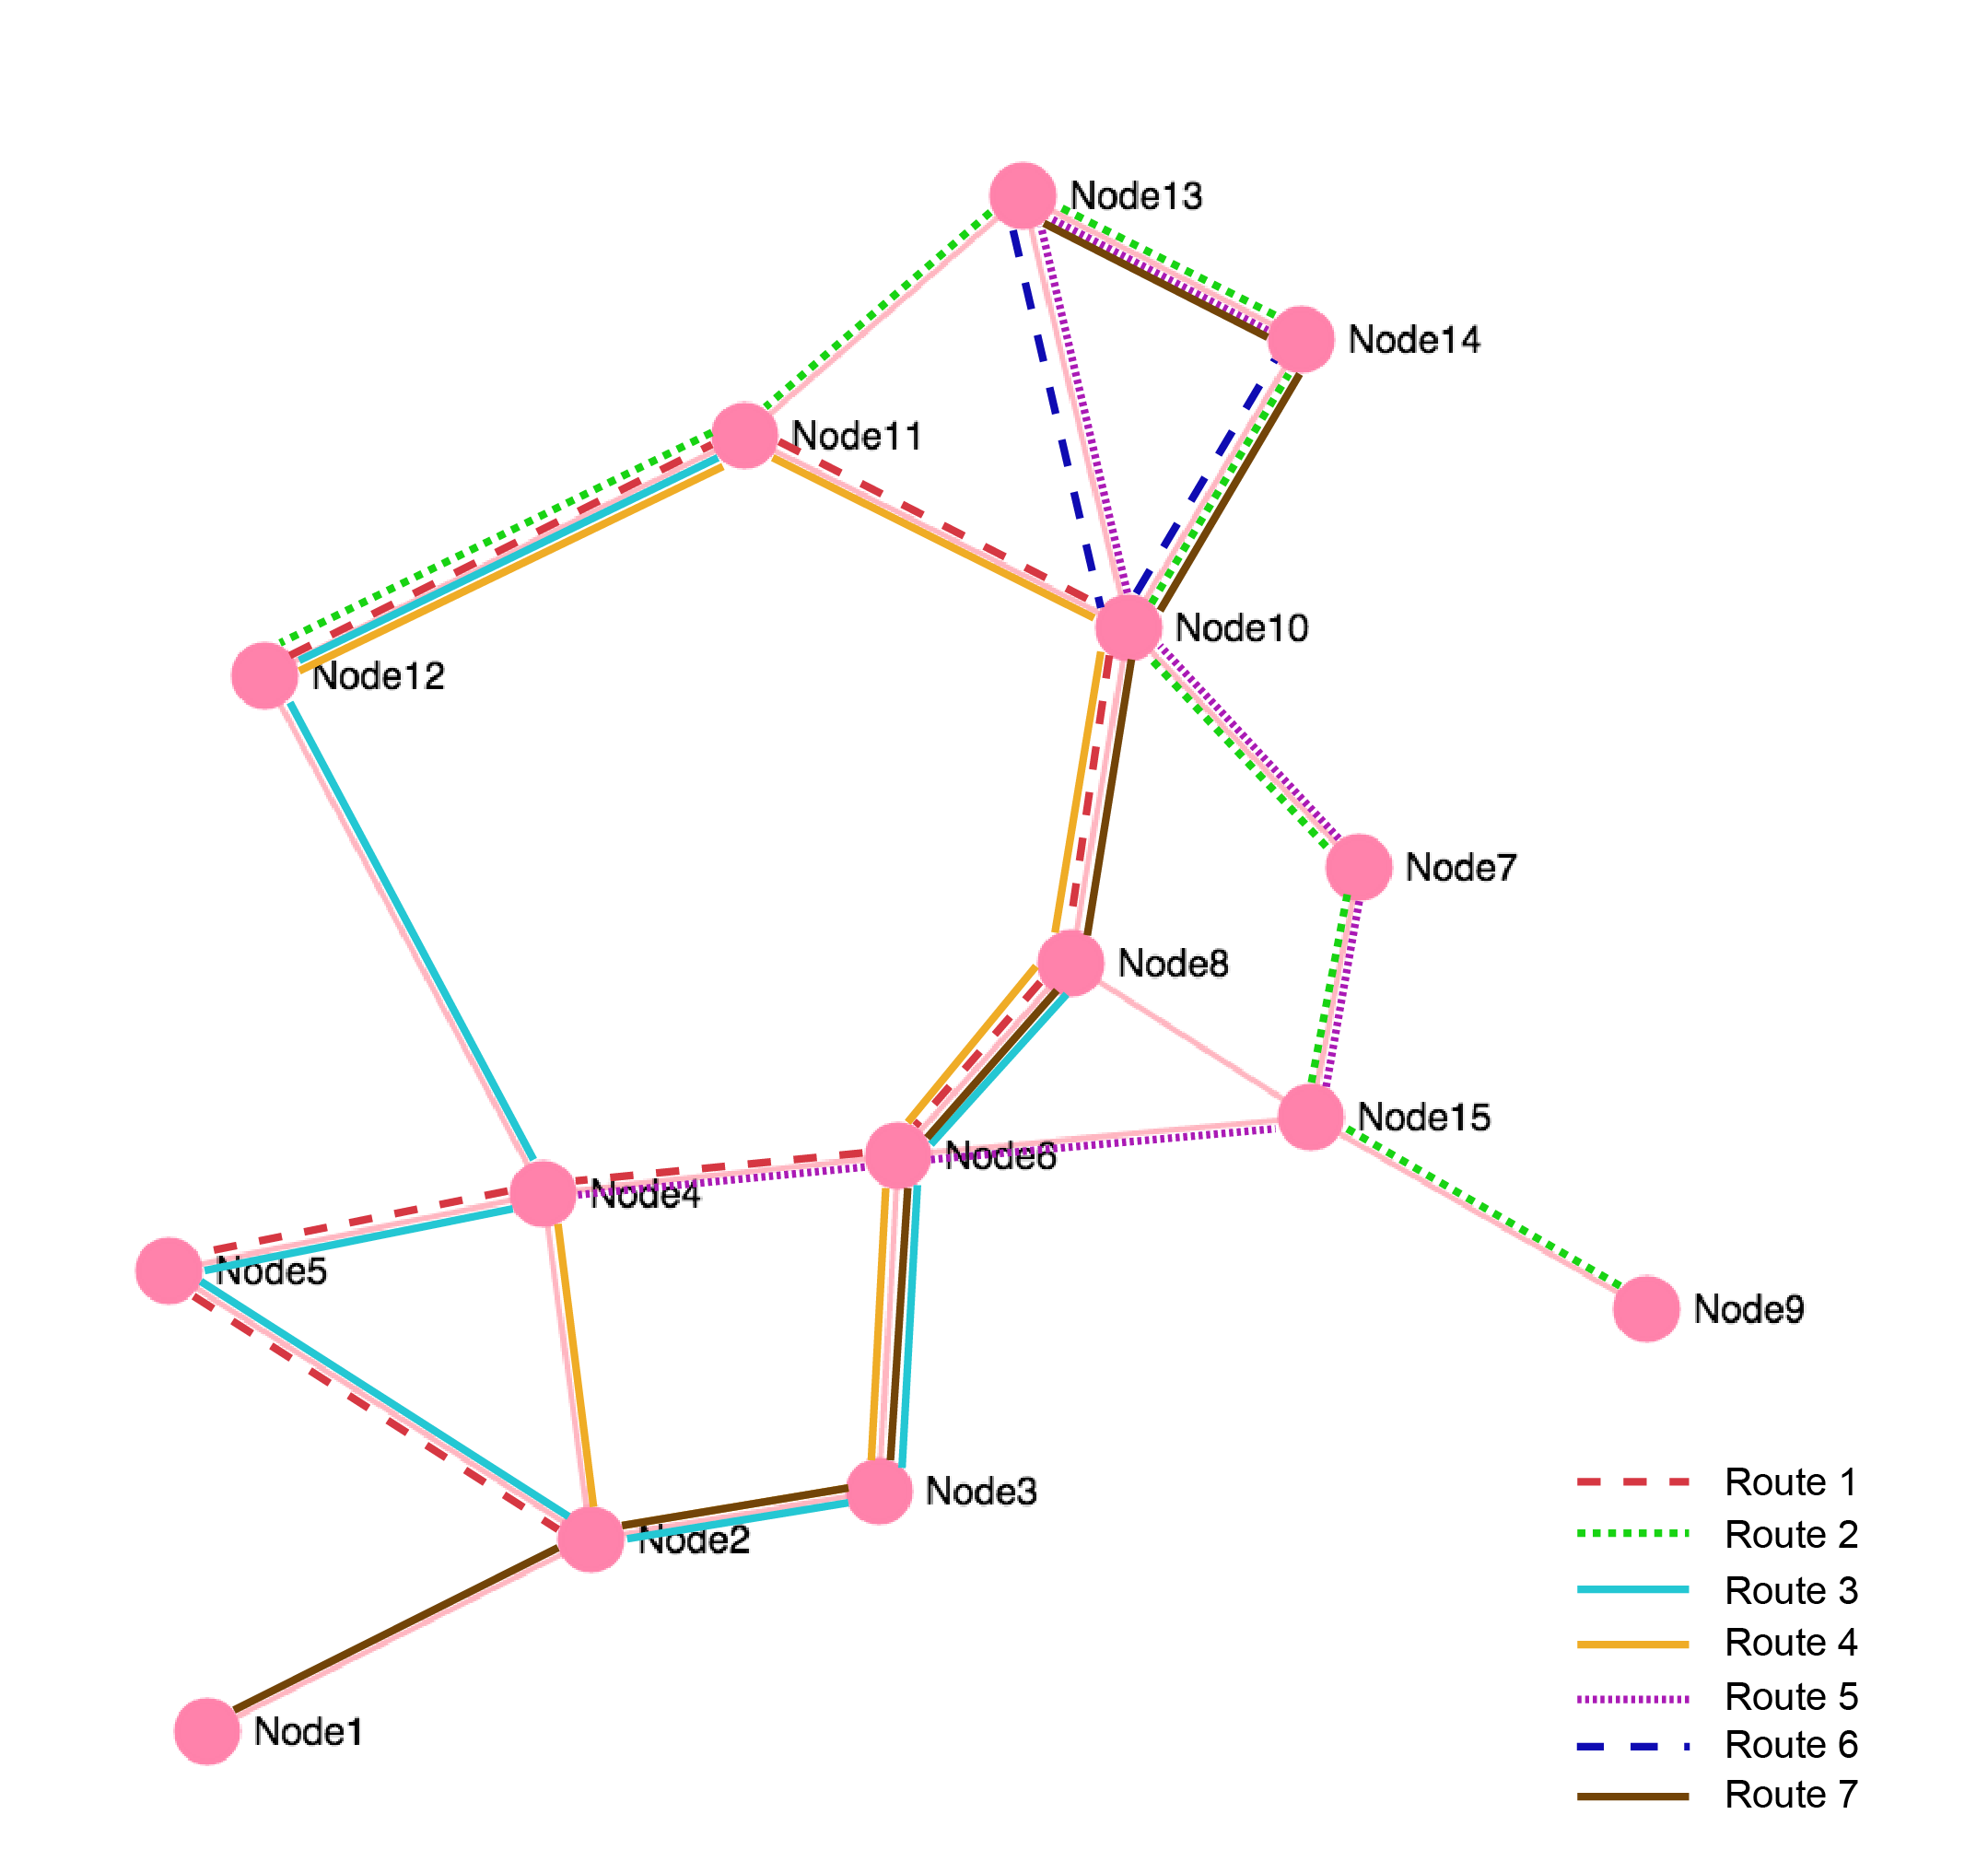
\includegraphics[width=4in]{assets/mandlnetwork_7routes.png}
    \end{center}
    \caption{Illustration of the best route set, having seven routes, constructed by the proposed system on Mandl's Network}
    \label{fig:bestRouteSet7} 
\end{figure}

\begin{table}[H]
    \centering
    \hspace*{-1.0cm}
    \begin{tabular}{|l||l|l|l|l|l|}
    \hline
    \textbf{System} & $d_0(\%)$ & $d_1(\%)$ & $d_2(\%)$ & $d_{unsat}(\%)$ & $ATT$ \\
    \hline
    \citet{nikolic14} & 94.41 & 5.59 & 0.00 & 0.00 & - \\
    \citet{chakroborty02} & 89.15 & 10.85 & 0.00 & 0.00 & 10.15 \\
    \citet{kechagiopoulos14} best & 97.17 & 2.83 & 0.00 & 0.00 & 10.16 \\
    \citet{kechagiopoulos14} avg & 96.55 & 3.45 & 0.01 & 0.00 & 10.23 \\
    \citet{chew12} best & 95.57 & 4.42 & 0.00 & 0.00 & 10.27 \\
    \citet{chew12} avg & 96.47 & 3.53 & 0.00 & 0.00 & 10.31 \\
    \citet{fan10} best & 93.32 & 7.13 & 0.32 & 0.00 & 10.42  \\
    \citet{zhang10} & 92.89 & 7.11 & 0.00 & 0.00 & 10.46 \\
    \citet{fan10} SA avg & 92.47 & 6.95 & 0.58 & 0.00 & 10.62 \\
    \citet{kidwai98} & 93.91 & 6.09 & 0.00 & 0.00 & 10.70 \\
    \citet{fan10} HC avg & 92.21 & 7.13 & 0.66 & 0.00 & 10.74 \\
    \citet{baaj91} & 80.99 & 19.01 & 0.00 & 0.00 & 12.50 \\
    \hline
    SSO Best & 89.85 & 8.67 & 1.48 & 0.00 & 10.03\\
    SSO Average & 88.49 & 10.72 & 0.79 & 0.00 & 10.08\\
    SSO Median & 88.12 & 10.92 & 0.90 & 0.00 & 10.03\\
    SSO Worst & 83.94 & 15.93 & 0.13 & 0.00 & 10.01\\
    Standard Deviation & 2.29 & 2.32 & 0.42 & - & 0.08\\
    \hline
    \end{tabular}
    \caption {Comparing the best route set, having seven routes, produced by the proposed system with route sets constructed by other approaches.}
    \label{table:performanceComparison_7}
\end{table}
%-------------------- 8 route sets ---------------------
Table \vref{table:performanceComparison_4} presents the results produced by the proposed system, having eight routes, and results from route sets constructed by other approaches. The table is sorted in ascending order with respect to the $ATT$ value.

\begin{figure}[H]
    \begin{center}
    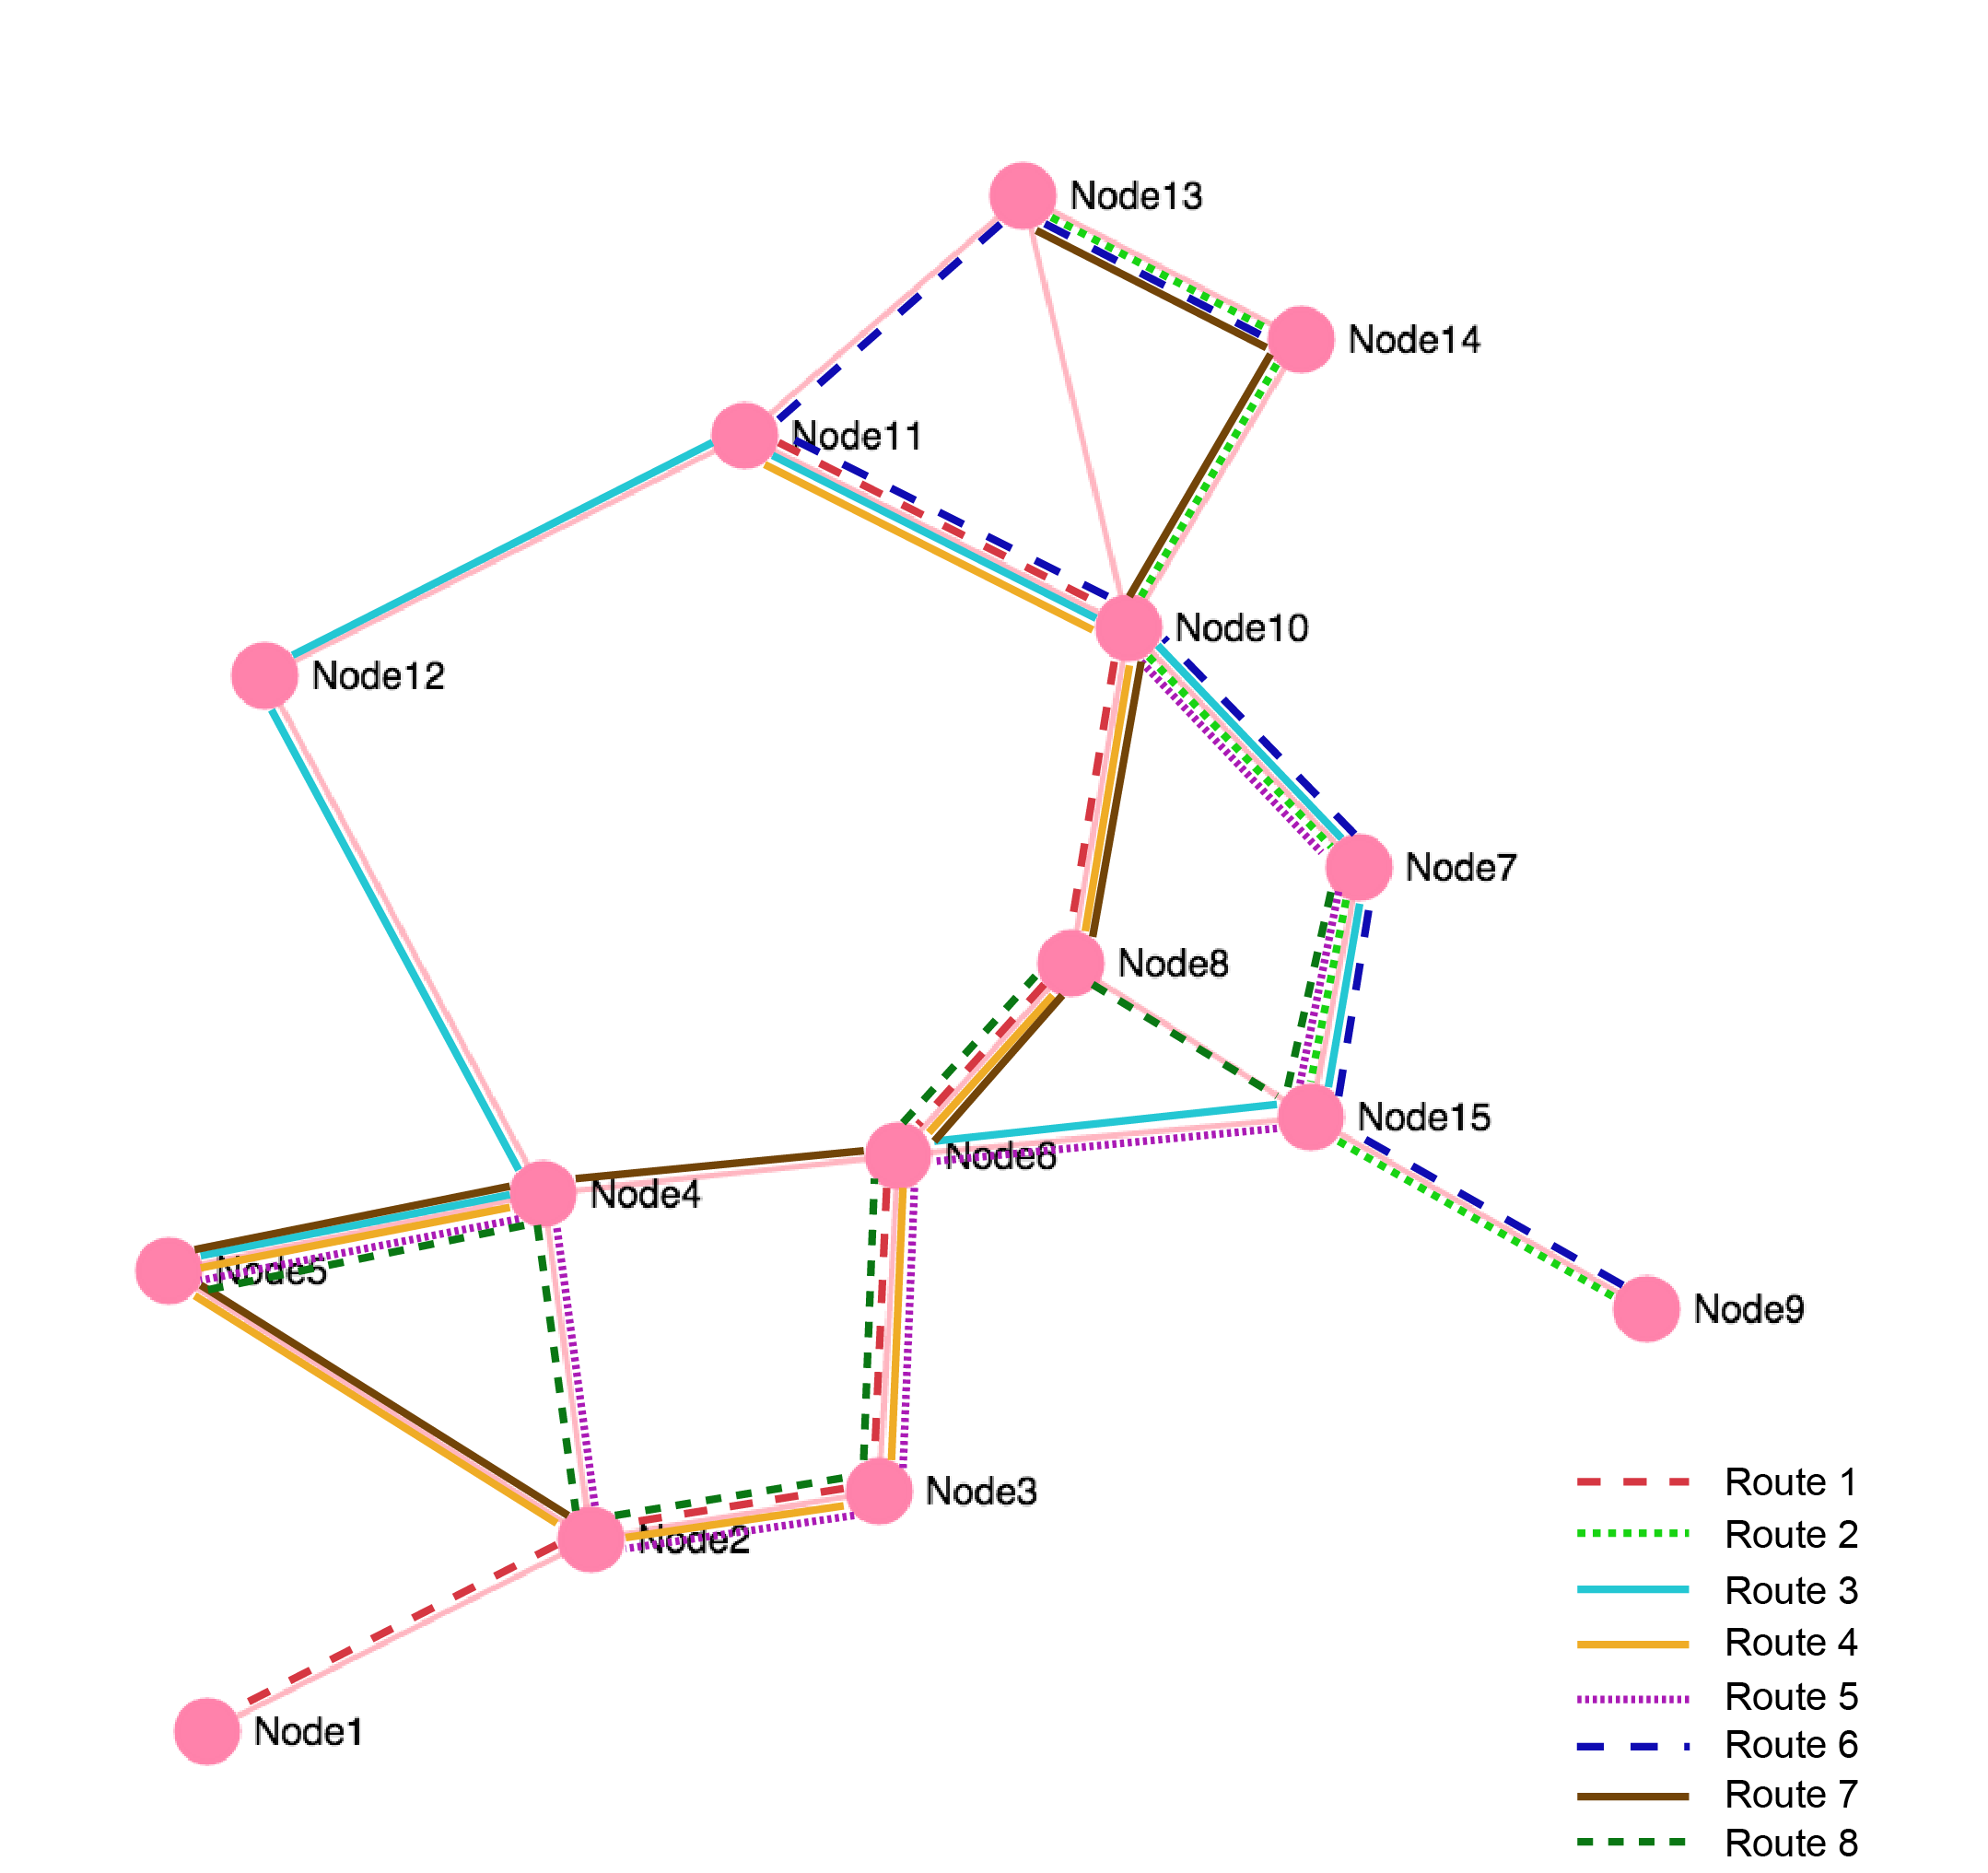
\includegraphics[width=4in]{assets/mandlnetwork_8routes.png}
    \end{center}
    \caption{Illustration of the best route set, having eight routes, constructed by the proposed system}
    \label{fig:bestRouteSet8} 
\end{figure}

    \begin{table}[H]
    \centering
    \hspace*{-1.0cm}
    \begin{tabular}{|l||l|l|l|l|l|}
    \hline
    \textbf{System} & $d_0(\%)$ & $d_1(\%)$ & $d_2(\%)$ & $d_{unsat}(\%)$ & $ATT$ \\
    \hline
    \citet{nikolic14} & 96.40 & 3.60 & 0.00 & 0.00 & - \\
    \citet{kechagiopoulos14} best & 97.75 & 2.25 & 0.00 & 0.00 & 10.13 \\
    \citet{kechagiopoulos14} avg & 97.47 & 2.53 & 0.00 & 0.00 & 10.17 \\
    \citet{chew12} best & 97.82 & 2.18 & 0.00 & 0.09 & 10.19 \\
    \citet{chew12} avg & 96.16 & 3.84 & 0.00 & 0.09 & 10.31 \\
    \citet{fan10} best & 94.54 & 5.46 & 0.00 & 0.00 & 10.36 \\
    \citet{zhang10} & 93.14 & 6.86 & 0.00 & 0.00 & 10.42 \\
    \citet{chakroborty02} & 90.38 & 9.58 & 0.00 & 0.00 & 10.46 \\
    \citet{fan10} Simulated Annealing & 93.65 & 5.88 & 0.47 & 0.00 & 10.58 \\
    \citet{fan10} Hill Climbing & 93.23 & 6.18 & 0.59 & 0.00 & 10.69 \\
    \citet{kidwai98} & 84.73 & 15.27 & 0.00 & 0.00 & 11.22 \\
    \citet{baaj91} & 79.96 & 20.04 & 0.00 & 0.00 & 11.86 \\ 
    \hline
    SSO Best & 91.01 & 7.9 & 1.09 & 0.00 & 10.01\\
    SSO Average & 89.16 & 10.05 & 0.8 & 0.00 & 10.06\\
    SSO Median & 88.7 & 10.21 & 0.77 & 0.00 & 10.03\\
    SSO Worst & 92.42 & 6.81 & 0.77 & 0.00 & 10.08\\
    Standard Deviation & 2.24 & 2.14 & 0.68 & - & 0.07\\
    \hline
    \end{tabular}
    \caption {Comparing the best route set, having eight routes, produced by the proposed system with route sets constructed by other approaches.}
    \label{table:performanceComparison_8}
    \end{table}

%---------------------- Execution time ---------------------



%Table \vref{table:performanceComparison_runtime} shows the average runtime for each run with 50 runs.

